
\section{Miscellany}
Condensed Matter (e.g., crystal
structure, x-ray diffraction, thermal
properties, electron theory of metals,
semiconductors, superconductors)
Miscellaneous (e.g., astrophysics, mathematical
methods, computer applications)

\subsection{Chemistry}

%%%%%%%%%%%%%%%%%%%%%%%%%%%%%%%%%

\subsection{Plasma}
\Table{
\hline

Debye length & $\lambda_D = \sqrt{ \dfrac{\epsilon_0 k_B T_e}{n_eq_e^2}} $

\\ \hline
}

\subsection{Condensed Matter} 

%%%%%%%%%%%%%%%%%%%%%%%%%%%%%%%%%

\subsection{Crystal structure} 

%%%%%%%%%%%%%%%%%%%%%%%%%%%%%%%%%

\subsection{X-ray diffraction} 
\center
\begin{tabular}{|c|c|}
\hline

Bragg Diffraction &

\begin{minipage}{0.6\textwidth}

 $n \lambda = 2d \sin \theta$ like a thin film, but using a different angle, i.e. the angle between the beam and the surface plane.
 
 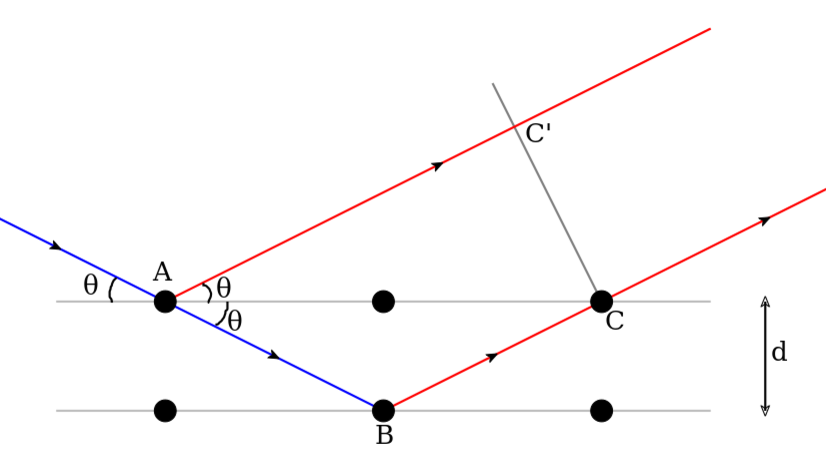
\includegraphics[width=75mm, height=50mm]{images/Bragg.png}
      \tiny \url{https://en.wikipedia.org/wiki/Bragg\%27s_law}
\end{minipage}

\\ \hline
\end{tabular}
\flushleft

\subsection{Thermal properties} 

%%%%%%%%%%%%%%%%%%%%%%%%%%%%%%%

\subsection{Electron theory of metals}
\center
\begin{tabular}{|c|c|}
\hline

\MiniPg{.4}{

At the highest energies of the valence band in many semiconductors (Ge, Si, GaAs, ...), and the lowest energies of the conduction band in some semiconductors (GaAs, ...), the band structure $E(\bold{k})$ can be locally approximated as

}

&
 
$E(\bold{k}) = E_0 + \dfrac{\hbar^2 \bold{k}^2}{2m^*}$
 
\\ \hline

\MiniPg{.4}{

Effective mass of electron in metals

}
 
& 

\MiniPg{.6}{
\center

\MPalign{
E & = \dfrac{\hbar^2 k^2}{2m} \\
\dfrac{dE}{dk} & = \dfrac{\hbar^2 k}{m} = \hbar v_g \\
\dfrac{dv_g}{dt} &= \dfrac{1}{\hbar} \dfrac{d^2E}{dt^2} \dfrac{dk}{dt} = \dfrac{1}{\hbar} \dfrac{d^2E}{dt^2} \dfrac{F}{\hbar} \\
F &= \hbar^2 \BigP{\dfrac{d^2E}{dt^2}}^{-1} \dfrac{dv_g}{dt} \\
m^* &= \hbar^2 \BigP{\dfrac{d^2E}{dt^2}}^{-1} 

}

}

\\ \hline
\end{tabular}
\flushleft

%%%%%%%%%%%%%%%%%%%%%%%%%%%%%%%%%


\subsection{Semiconductors}
\Table{
\hline

\MiniPg{.3}{\center
$n$-doped semiconductor
}

&

\MiniPg{.7}{\center
$n$ stands for negative, so $n$-type silicon is doped with negatively charged atoms (say, phosphorus) . This means that these atoms have extra electrons, and can easily part with the extra electron. Hence, they are donors.
}

\\ \hline
}

%%%%

\Table{
\hline

\MiniPg{.3}{\center
$p$-doped semiconductor
}

&

\MiniPg{.7}{\center
$p$ stands for positive, so $p$-type silicon is doped with positively charged atoms (say, boron). This means that these atoms have missing electrons, so they can easily accept new electrons to fill the vacancy. Hence, they are acceptors.
}

\\ \hline
}

%%%%%%%%%%%%%%%%%%%%%%%%%%%%%%%%%

\subsection{Superconductors} 

%%%%%%%%%%%%%%%%%%%%%%%%%%%%%%%%%

\subsection{Astrophysics} 

\Table{
\hline

Schwarzschild radius

&

$R = \dfrac{2MG}{c^2}$

\\ \hline
}

%%%%%%%%%%%%%%%%%%%%%%%%%%%%%%%%%

\subsection{Mathematical methods}

%%%%%%%%%%%%%%%%%%%%%%%%%%%%%%%%%

\subsection{Computer applications}



